\documentclass{standalone}
\usepackage{hsbcommon}
\begin{document}
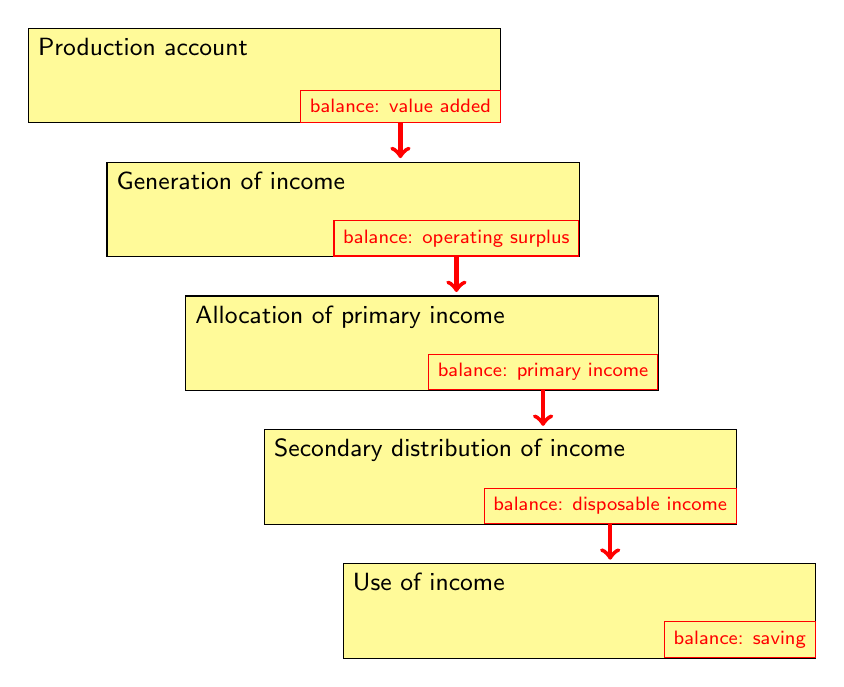
\begin{tikzpicture}
    \def\mystretch{1.7}
    \tikzset{
        myaccount/.style={
            draw,
            fill=yellow!40,
            font=\small\sffamily
        } 
    }
    \foreach[count=\i] \myaccount/\mybalance in 
        {%
        Production account/value added,
        Generation of income/operating surplus/mixed income,
        Allocation of primary income/primary income,
        Secondary distribution of income/disposable income,
        Use of income/saving%
        }
        {
            \draw[myaccount] (\i,-\mystretch*\i) 
                node[below right] (A\i) {\myaccount}
            rectangle (6+\i,-\mystretch*\i-1.2)
                node[above left,draw,red] (B\i) {\scriptsize balance: \mybalance}
            ;
        }
    \foreach \i in {1,...,4}
        \draw[->,red,ultra thick] (B\i.south) -- ++(0,-0.45);
        
\end{tikzpicture}
\end{document}